
\section{实验结果与测试}

\subsection{实验结果} \label{sec:r:result}

将第 \ref{sec:dcfgconv} 节的算法 \ref{alg:eg:dfgllvm} 实现之后,
对第 \ref{sec:codeeg} 节的图 \ref{fig:eg:code} 所示的示例代码
执行得到如图 \ref{fig:eg:result} 所示的图形。

\newsavebox{\egresult}
\sbox{\egresult}{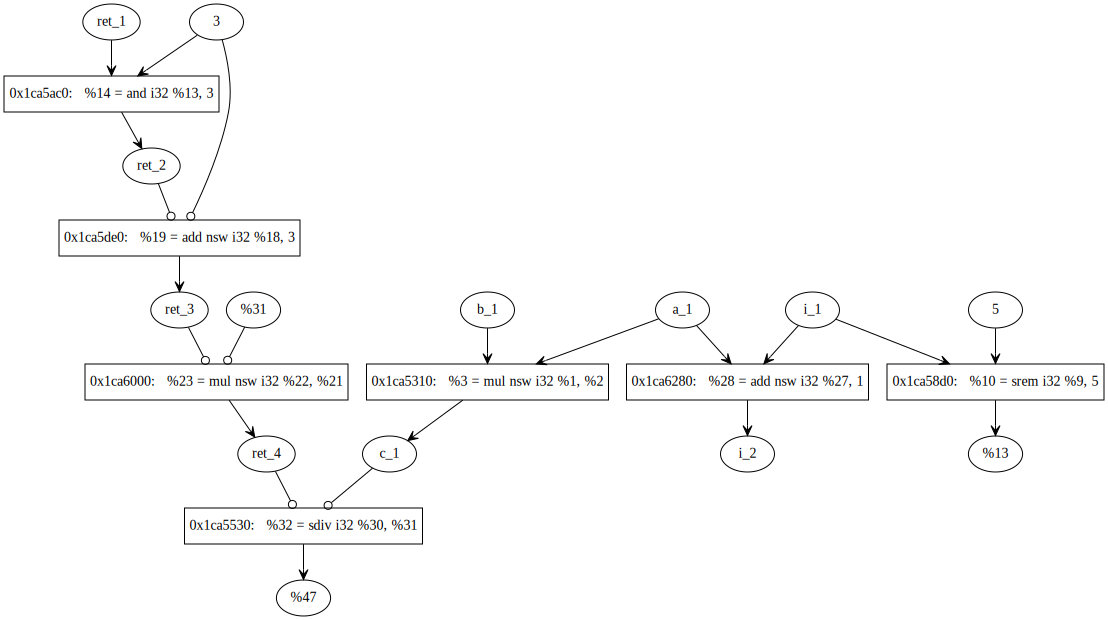
\includegraphics[width=14.6cm]{image/result.pdf}}
\begin{figure}[!hbt]
\centering
\usebox{\egresult}
\caption{代码E的实验结果} \label{fig:eg:result}
\end{figure}

图 \ref{fig:eg:result} 的具体dot源文件如下所示:

{
    \setstretch{1.0}
    \lstinputlisting[style=lstnone]{code/func.dot}
}

\subsection{其他测试与BUG}

在改变多种输入后发现,本生成工具还存在如下问题:

{
\setstretch{1.0}
\begin{itemize}
    \addtolength{\itemindent}{2.5em}
    \item 函数相关的Call指令已经成功解析并加入图中,但在打印时没能打印出和它相连的边。
    \item 对于源代码中的常量,程序对其名称的获取依然会失败。
    \item 对于匿名的虚拟寄存器,程序未能对其识别并赋与独立的名字。
\end{itemize}
}

因此,本工具的功能还需进一步加强。